
\chapter{Aplicação e Resultados} \label{chap:4}


\section{O Simulador Pipesim}
Sistemas de produção de petróleo são sistemas nos quais se deseja sempre produzir o máximo possível e de forma segura.
O PIPESIM, da Schlumberger, é um simulador de fluxo multifásico em regime permanente que pode ser utilizado tanto para o projeto como para planejamento de operações em campos de petróleo. Ele permite que sejam simuladas situações alternativas de forma mais rápida e segura que testes reais.

\section{Python}

O Python é uma linguagem de alto nível, interpretada, de desenvolvimento rápido muito utilizada para prototipação e na academia. Suas faciliades, como Jupyter Notebook, um ambiente que facilita a criação de documentos com códigos e análise de dados, e o Matplotlib, uma biblioteca que a torna quase tão poderosa quando o MatLab para visualização de dados, a tornaram muito utilizada também na academia.

A Linguagem surgiu em 1991, e segundo o toba [https://www.tiobe.com/tiobe-index/] é a quarta linguagem de programação mais popular atualmente.

Sua facilidade de uso, expêriencia prévia, e facilidades de visualização de dados foram decisivos para a sua escolha para este trabalho. 

\section{Interface Python e OpenLink}
Para interfaceamento do Pipesim com outros softwares, a Schlumberger disponibiliza uma API (Application Programming Interface) chamada OpenLink, idealizada para programação em C++, VBA, ou Visual Basic. Esta pode ser utilizada para interação programática com o Pipesim, habilitando a configuração de novos poços, alteração de poços existentes, análises, simulações, e automação de simulações. Com essa API, é possível variar os parametros do poço e avaliar as curvas características.

 Utilizando-se a biblioteca de Python pyWin32, é possível comunicar-se com a API, mas apenas em versões do Windows de 32 bits. Apesar de algumas peculiaridades no tratamento de arrays e outros tipos de dados, esta biblioteca permite o uso da API em uma linguagem de desenvolvimento mais rápido[citation needed] e com grandes facilidades de análise de dados [citation needed].

\section{NOMAD}
Para utilização do orthoMADS, foi escolhida a ferramenta NOMAD, uma implementação em C++ para a solução de problemas de otimização sem-derivadas com problemas caixa-preta, aonde não se conhece o modelo explícito do problema. Bastando fornecer uma função objetivo e restrições, a ferramenta é capaz de encontrar um ponto ótimo para o problema. Ela também  disponibiliza variações do algorítmo (como 2n ou n+1 bases) e a possibilidade de paralelismo (consultar mais que um ponto de forma concorrente.  


\section{Opal}
Para o uso do NOMAD com o Python, era sugerido, até o começo destes trabalhos, o uso da ferramenta Opal (A Framework for Optimization of Algorithms). Uma interface open-source de alto nível para a interface de Python com o NOMAD. Este framework dá a liberdade para configurar todos os parametros de otimização do NOMAD e também é capaz de paralelismo.

No entanto ele suporta apenas Python2.7 que está em desuso há mais de 10 anos [citation needed], de modo que foi necessário portá-lo para python3 [github], contribuição que foi enviada aos criadores originais [action needed].



\section{Experimentos}
Foi realizado um experimento de sintonia de curva, e utilizadas três abordagens diferentes para a sintonia. Primeiramente foi utilizado o orthoMADS, com a implementação NOMAD, em seguida, foi utilizado novamente o NOMAD, mas com surrogate model calculado pela SGTELIB, e finalmente, uma implementação do Nelder-Mead Simplex. Os resultados então são comparados quanto a número de avaliações e acuracia do resultado.

\section{O Problema de sintonia}
Primeiramente foi configurado um unico poço de petróleo, que pode ser visto na figura \ref{fig:setup1_dia}. A seguir foram escolhidos dados arbitrariamente para compor a curva "real" de produção (figura \ref{fig:truth1}).
Neste Experimento a curva sintonizada foi a de fluxo de líquido (Barris padrões por dia) por gás injetado (milhões de pés cúbicos padrões por dia). Escolheu-se a pressão estática do reservatório como sendo 4000 psi absoluto, e um indice de produtividade liquido de 25 STDB/d/psi( Barris padrões por dia por pressão estática). Desta forma a figura \ref{fig:truth1} demonstra a curva "real" a ser sintonizada.



\begin{figure}
\centering
\begin{subfigure}{.4\textwidth}
  \centering
  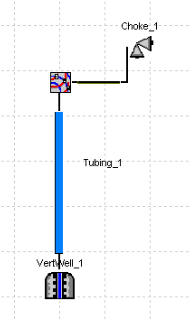
\includegraphics[height=1\linewidth]{figs/setup1.png}
  \caption{Setup do poço de petróleo.}
  \label{fig:setup1_dia}
\end{subfigure}%
\begin{subfigure}{.6\textwidth}
  \centering
  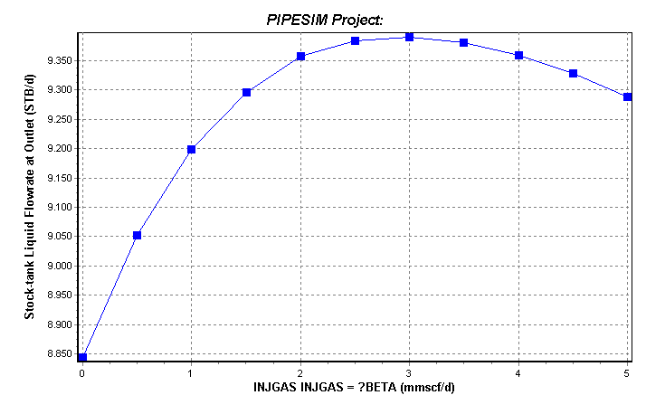
\includegraphics[height=0.7\linewidth]{figs/truth1.png}
  \caption{Curva "real" do poço de petróleo.}
  \label{fig:truth1}
\end{subfigure}
\caption{Experimento 1.}
\label{fig:setup1}
\end{figure}

Para os testes, os parametros SP (pressão estática) e Liq PI (Índice de produção de líquido) foram iniciados respecticamente em 3000 e 15. A interface OpenLink foi utilizada para modificar os parâmetros e ler uma nova curva, a distância quadrática entre as duas curvas foi utilizada como o erro na otimização.

\section{Setup para sintonia de curva com o orthoMADS}
Para a sintonia com o orthoMADS, foi utilizada o framework OPAL (A Framework for Optimization of Algorithms), interface python para o solver NOMAD.
A implementação com o OPAL utiliza dois arquivos, "well\_declaration.py" e "well\_optimize.py".

O arquivo "well\_declaration.py" expõe os componentes do problema:

\begin{itemize}
\item Nome do algoritmo:
\begin{verbatim}
# Define Algorithm object.
tuning = Algorithm(name='TUNING', description='Well Tuning')
\end{verbatim}
\end{itemize}

\begin{itemize}
\item Comando utilizado pelo solver para avaliar a função:
\begin{verbatim}
tuning.set_executable_command('python pipesim_run.py')
\end{verbatim}
\end{itemize}


\begin{itemize}
\item As variáveis de decisão:
\begin{verbatim}
static_pressure = Parameter(kind='real', 
                            default=sp, 
                            bound=(2000, 7000),
                            name='sp', 
                            description='Static Pressure')
liq_pi = Parameter(kind='real', 
                   default=pi, 
                   bound=(15, 35),
                   name='pi', 
                   description='Liq PI')

FD.add_param(static_pressure)
FD.add_param(liq_pi)
\end{verbatim}
\end{itemize}

\begin{itemize}
\item E o erro:
\begin{verbatim}
error = Measure(kind='real', name='ERROR', description='Curve quadratic error')
FD.add_measure(error)
\end{verbatim}
\end{itemize}

Já no arquivo "well\_optimize", são declaradas estruturas auxiliares, e instanciado o solver

\begin{verbatim}

def get_error(parameters, measures):
    return sum(measures["ERROR"])

data = ModelData(FD)
struct = ModelStructure(objective=get_error)  # Unconstrained
model = Model(modelData=data, modelStructure=struct)

NOMAD = NOMADSolver()

\end{verbatim}



Adicionalmente, são impostas as seguintes restrições ao solver do NOMAD:
\begin{verbatim}
F_TARGET = 0.1
\end{verbatim}

De modo a limitar o tamanho mínimo da malha, e terminar a simulação quando a função custo chegar a um valor abaixo de 0.1

E a seguir, é inicilizada a otimização:
\begin{verbatim}
NOMAD.solve(blackbox=model)
\end{verbatim}


\section{Resultados da Sintonia de Curva com o orthoMADS}

Em 525 segundos (8:45 minutos) e necessitou de 206 avaliações de caixa preta. O NOMAD convergiu para SP=4000.691, PI = 24.9544, com a função custo em 0.0757. A parada se deu pelo F\_TARGET. A performance do algoritmo pode ser vista na figura \ref{fig:setup1_2}.


\begin{figure}
\centering
\begin{subfigure}{0.5\textwidth}
  \centering
  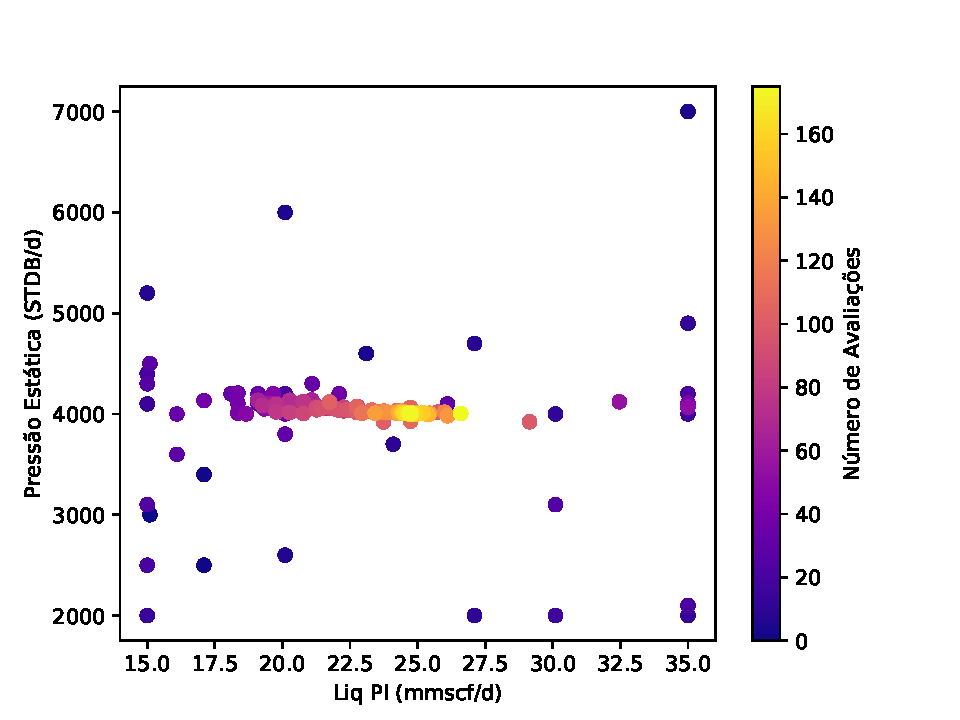
\includegraphics[width=1\linewidth]{figs/setup1_eval_points.pdf}
  \caption{Pontos escolhidos pelo NOMAD.}
  \label{fig:setup1_points}
\end{subfigure}%
\begin{subfigure}{0.5\textwidth}
  \centering
  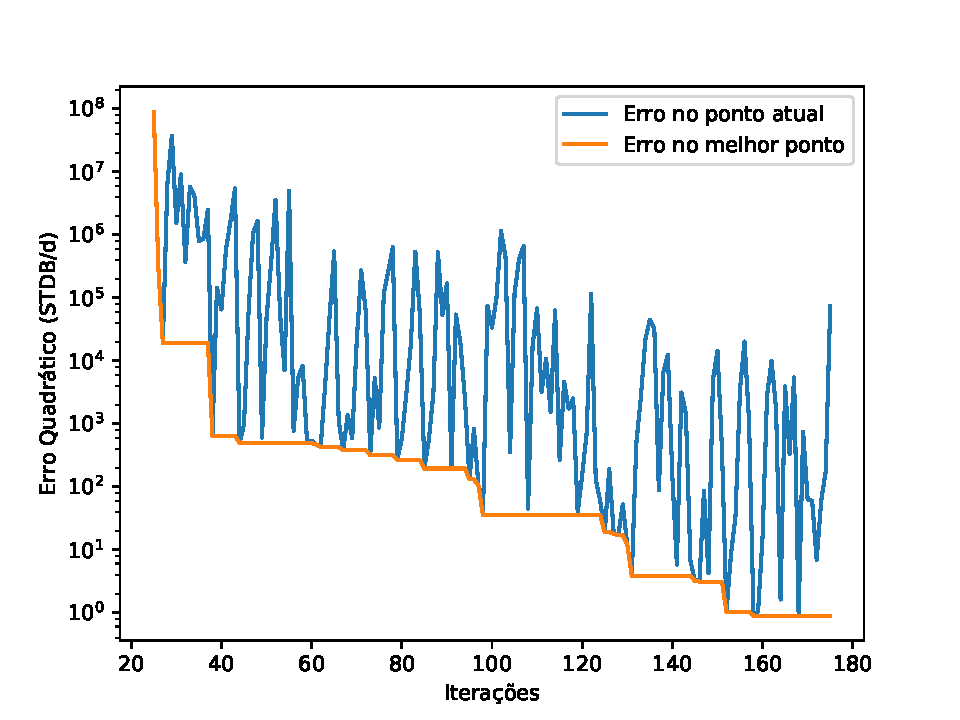
\includegraphics[width=1\linewidth]{figs/setup1_errors.pdf}
  \caption{Erro nos pontos avaliados.}
  \label{fig:setup1_error}
\end{subfigure}
\caption{Experimento 1.}
\label{fig:setup1_2}
\end{figure}

\section{Surrogate Lib}

Durante a realização desses experimentos, o NOMAD foi atualizado e recebeu uma ferramenta auxiliar, uma biblioteca que tenta aproximar a função a partir dos pontos já utilizados, para utilização no passo "search" do algoritmo. Esta biblioteca faz com que o algoritmo, a cada iteração, tente adivinhar a melhor direção para avançar, ao invés de progredir aleatoriamente.

Para o cálculo do modelo substituto, são possíveis nove tipos de modelos, que podem ser vistos na documentação, além de onze tipos possíveis de núcleos. Neste trabalho foram utilizadas as opções padrão do NOMAD, um modeo PRS (Polynomial Response Surface) de ordem 2.


\section{Setup Para Sintonia de Curva Com a Surrogate Lib}

Um contra-tempo quanto a SGTELIB, como é chamada a biblioteca, é que ela está embutida nos binários do NOMAD, e, por algum erro, os binários para windows foram compilados com uma versão antiga do Microsoft Visual Studio, de forma que é necessário recompilar não apenas o sgtelib (o que pode ser feito com o mingW sem grandes mudanças), mas todo o NOMAD, necessitando a instalação de aproximadamente 4Gb do Visual Studio.

Após sua recompilação, bastou substituir o binário antigo pelo novo, é inserir nos parâmetros do NOMAD para o uso da SGTELIB, com seus valores padrõess:
\begin{verbatim}
NOMAD.set_parameter(name="MODEL_SEARCH", value="SGTELIB")
\end{verbatim}
Para que ele passasse a utilizar o SGTELIB no local do seu SEARCH baseado em modelo quadrático.


\section{Resultados da Otimização Com a Surrogate Lib}

A execução demorou 1374 segundos (22:27 minutos) e necessitou de 417 avaliações de função de caixa preta. O Nomad novamente convergiu, para $SP=4001.389, Liq PI =24.905$, com uma função custo de 0.09986.

é possível notar, no entanto, que com o SGTELIB, em muitos pontos o erro quadrático saturou em $10^{64}$. Nota-se também que pontos longe do ótimo foram avaliados perto da convergência (pontos claros no canto inferior esquerdo), o que pode significar que existe um problema com a SGTELIB, ou que o modelo utilizado não é o ideal.

\begin{figure}
\centering
\begin{subfigure}{0.5\textwidth}
  \centering
  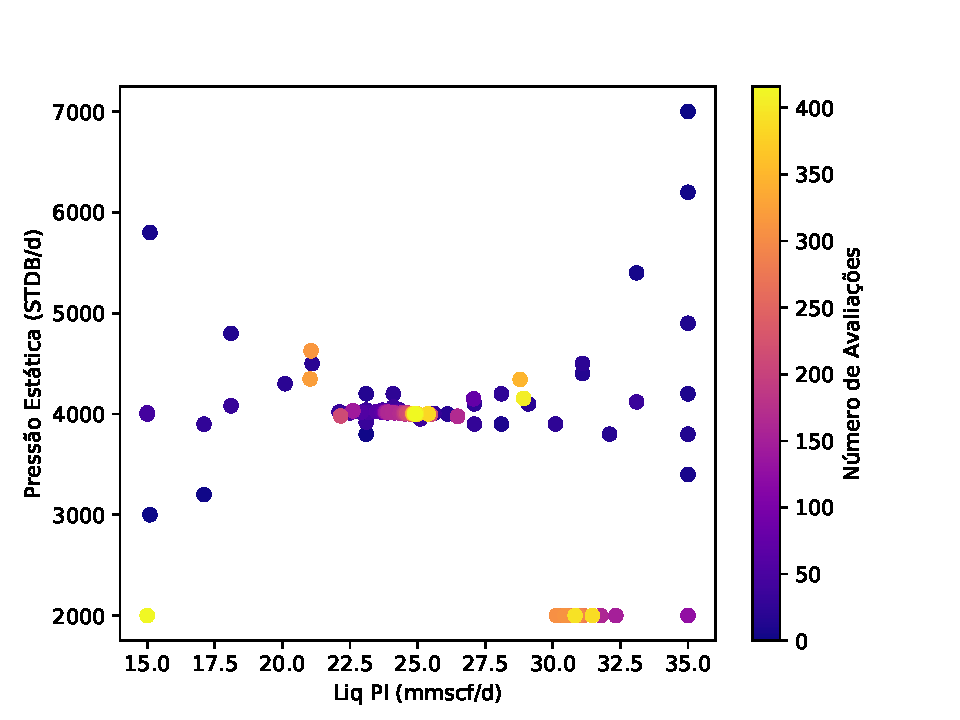
\includegraphics[width=1\linewidth]{figs/setup1sgtelib_eval_points.pdf}
  \caption{Pontos escolhidos pelo NOMAD.}
  \label{fig:setup2_points}
\end{subfigure}%
\begin{subfigure}{0.5\textwidth}
  \centering
  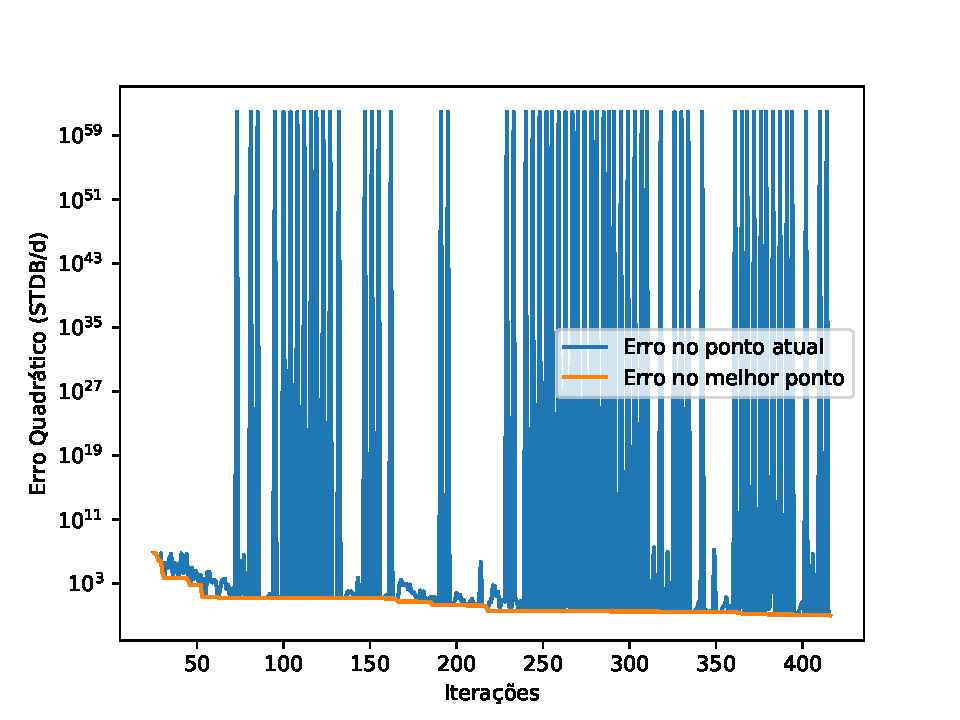
\includegraphics[width=1\linewidth]{figs/setup1sgtelib_errors.pdf}
  \caption{Erro nos pontos avaliados.}
  \label{fig:setup2_error}
\end{subfigure}
\caption{Experimento 1 com SGTELIB.}
\label{fig:setup2_2}
\end{figure}


\section{Setup da Otimização com Nelder-Mead Simplex}

Para o teste com o Simplex de Nelder-Mead, foi utilizada uma implementação pŕopria, baseada no \ref{alg:nm}, e como o algoritmo não é facilmente paralelizável, não houveram preocupações com paralelismo.
os limites utilizados foram os mesmos dos casos anteriores:
\begin{align}
15 < &pi < 35 \\
2000 < &sp < 7000
\end{align}

Como o simplex utiliza uma estrutura n-dimensional para a busca, são necessários n+1 pontos iniciais, por este motivo um triângulo foi expandido arbitrariamente a partir do ponto inicial, de modo que no começo do algoritmo, o simplex inicial seja grande. 

as restrições foram aplicadas somando-se um peso adicional a função custo.

Os resultados podem ser vistos nas figuras \ref{fig:setup3_2} e \ref{fig:setup3_triang}. Nota-se que a solução foi mais rápida, com 212 iterações em 133 segundos (2:13 minutos). No entanto, o método de Nelder e Mead não tem a mesma garantia de convergência que os os métodos MADS. É interessante comentar a o caso da figura 5, aonde é possivel notar que o simplex primeiramente contraiu-se por um lado, gerando a parte roxa, depois contraiu-se do outro, até chegar ao ponto ótimo.



\begin{figure}
\centering
\begin{subfigure}{0.5\textwidth}
  \centering
  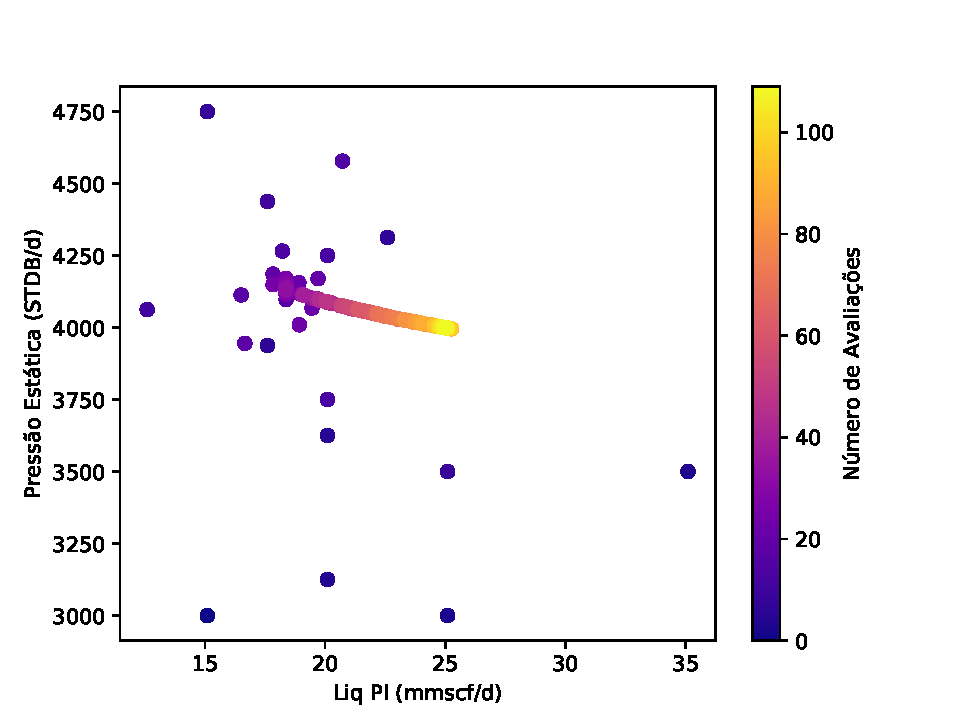
\includegraphics[width=1\linewidth]{figs/setup1nm_eval_points.pdf}
  \caption{Pontos escolhidos pelo Nelder-Mead.}
  \label{fig:setup3_points}
\end{subfigure}%
\begin{subfigure}{0.5\textwidth}
  \centering
  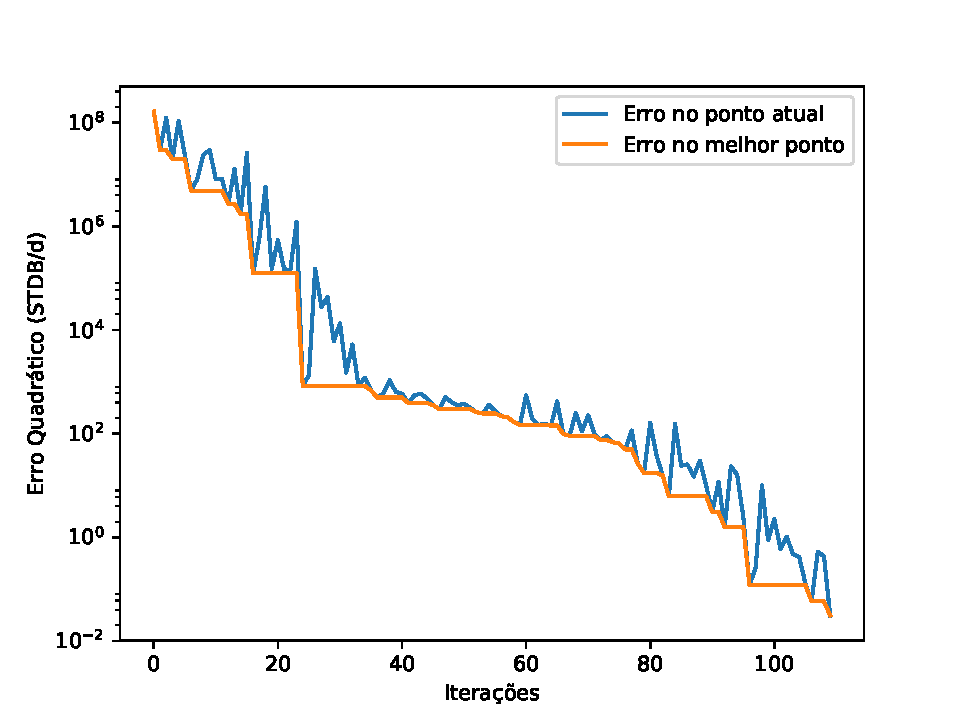
\includegraphics[width=1\linewidth]{figs/setup1nm_errors.pdf}
  \caption{Erro nos pontos avaliados.}
  \label{fig:setup3_error}
\end{subfigure}
\caption{Experimento 1 com Nelder-Mead.}
\label{fig:setup3_2}
\end{figure}

\begin{figure}
\centering
  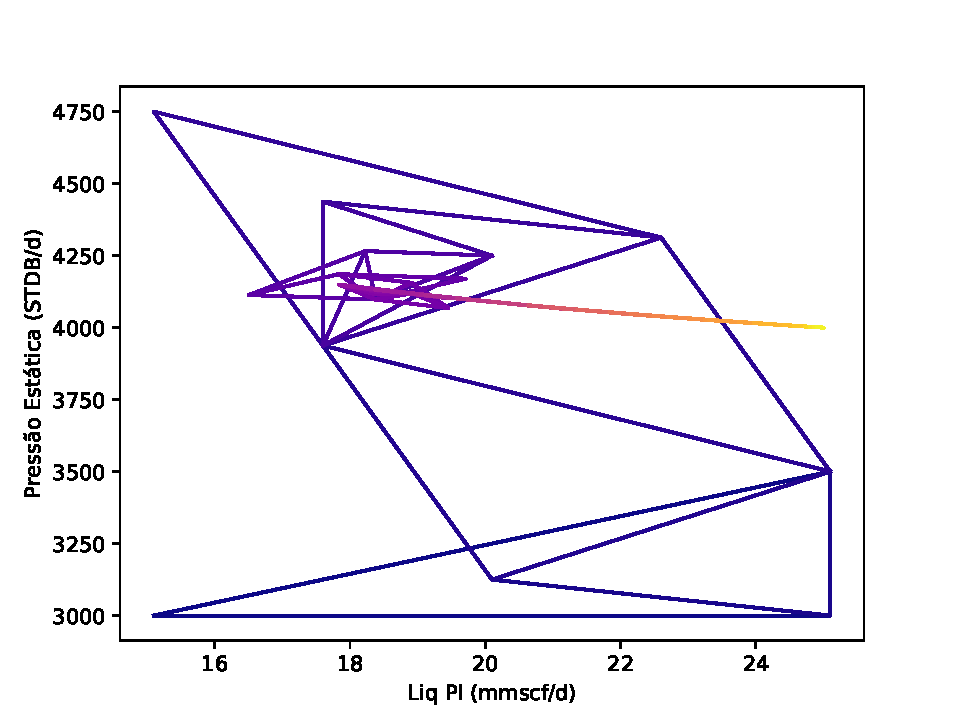
\includegraphics[width=0.7\linewidth]{figs/triangles_neldermead.pdf}
  \caption{Simplexes utilizados pelo Nelder-Mead.}
  \label{fig:setup3_triang}
\end{figure}




\section{Discução}





%%%%%%%%%%%%%%%
